\documentclass[a4paper]{scrartcl}

\usepackage[square,numbers]{natbib}
\usepackage[english]{babel}
\usepackage{booktabs}
\usepackage{graphicx}
\usepackage{url}
\usepackage[T1]{fontenc}

\begin{document}
	
\pagenumbering{gobble}

\begin{titlepage}
	\begin{center}
		\vspace*{1cm}
		
		{\LARGE \textbf{Title}}
		
		\vspace{0.5cm}
		
		{\LARGE Title complement}
		
		\vspace{1.5cm}
		
		\textbf{Author(s) : First Name LAST NAME}
		
		\vspace{0.5cm}
		
		\textbf{Supervisor: First Name LAST NAME}
		
		\vfill
		
		State-of-the-Art for the Course\\
		Introduction to the Scientific Approach [IHDCB339]\\
        Prof. Pierre-Yves Schobbens \& Julien Albert 	
		
        \vspace{0.8cm}
        
		
\includegraphics[width=0.3\textwidth]{figures/unamur}
  
		Faculty of Computer Science\\
		University of Namur\\
		Belgium\\
		May 2024
	\end{center}
\end{titlepage}
\newpage
\begin{center}
	\textbf{Abstract}
\end{center}
%% DELETE FROM HERE
%%
%% Template Presentation and Abstract 
% explain the purpose of this document, and the fact that the proposed structure does not have to be followed and can be modified.

This document is a template designed to help you write your state-of-the-art. It proposes a typical structure for your work, as well as a description of the various parts expected. This structure can, of course, be amended as required.
The guidelines for the content in this document are complementary to the guidelines for the execution of the work presented in the student compendium.
Finally, in the appendix you'll find a brief introduction to \LaTeX, outlining the features you'll need to write your state-of-the-art report.

NB: When using this template, this part must of course be deleted (lines 52-70 in the \texttt{main.tex} file).
\vskip1cm
The abstract is a summary of your state-of-the-art. Its purpose is to give the potential reader an idea of the content of the manuscript and to assess its interest. It begins with a presentation of the subject and the problem you are addressing. It then briefly describes your contribution. Finally, it highlights its impact on the research topic. A good abstract doesn't have to be long - 150-200 words is usually enough. If you'd like to find out more about writing an abstract, take a look at \cite{abstract}.
\vskip1cm
\begin{center}
	\textbf{Résumé}
\end{center}
Dans notre Faculté, on rédige le résumé en anglais ET en français, indépendemment de la langue de rédaction du document lui-même, qui est normalement l'anglais (OU le français moyennant acceptation par le promoteur). Nous avons donc rédigé le reste du document en anglais.

%% DELETE UNTIL HERE

\newpage

\tableofcontents

\newpage

\pagenumbering{arabic}

%%
%% Text Body
%%
%% INTRODUCTION
%%
\section{Introduction}

The introduction begins by introducing the field of research by contextualizing it and introducing main concepts. You will also highlighting some of the different currents and issues. Through this funneling process, you must arrive at your research topic, which will be described in the next section. One or more well-chosen examples to illustrate the issue and enable the reader to grasp its importance and interest could definitely help.

The purpose of the introduction is also to convince the reader that your work is worth reading. It should therefore be stressed that the problem is important and the contribution appropriate~\cite{melot2008elements}.
Finally, it's important to keep in mind that the reader doesn't necessarily know the subject and/or isn't an expert in the field~\cite{melot2008elements}.

Finally, the introduction is also the moment when the general plan of the manuscript is presented.

%%
%% PROBLEM STATEMENT
%%
\section{Problem Statement}

This part is mainly an adaptation of the problem state submitted for the January session.

\subsection{Research Field}

This section introduces the research field. First, it familiarizes the reader with the field by introducing the basic concepts and locating it in computer science. It then highlights the different trends and issues that make up research in the field.

\subsection{Research Topic}

You will begin by presenting your research topic more specifically. In addition to the presentation itself, you'll need to justify its relevance and interest in the context of your research field (why is it important?). This involves discussing existing solutions and their limitations~\cite{melot2008elements}.

\subsection{Problem Statement}

The research topic will then be formulated in the form of one or more research questions that define the scope of your work. These questions must, of course, be justified in terms of the subject and, more generally, the research area. But you also need to show that a literature review addressing those research questions is relevant.

%%
%% METHODOLOGY
%%
\section{Methodology}

The goal here is to explain how you are going to proceed to collect and analyze scientific literature to answer the research question(s).
In addition to a description of the methodology itself, which should make it possible to replicate the work carried out, the relevance of the choices made to the subject in question should be highlighted.
Finally, you must describe the conditions under which this work was carried out. If applicable, you should indicate whether and how you used artificial intelligence tools. This applies to article search, content extraction and analysis, and manuscript writing.

\subsection{Literature Research}

This section presents the bibliographical research methodology used to build up the corpus of references analyzed later.
In particular, we need to show that the methodology used has ensured that the references collected are representative of the research question.

The first step is to present the sources consulted, i.e., mainly bibliographic databases, and why they were chosen. 
Next, you'll need to present the search query(s) used, showing that they allow you to find a maximum number of relevant articles while limiting irrelevant references. To do this, you'll need to explain the different concepts manipulated and the keywords chosen.
Finally, where appropriate, other complementary methods can also be presented, explaining why they were used.

\subsection{Literature Selection}

This section describes and justifies the inclusion/exclusion criteria used for the selection of the relevant references. It also describes the selection process itself, in particular the number of references at the beginning and at the end.

\subsection{Extraction \& Analysis}

This section is dedicated to the tools and techniques used to extract and analyze information from your selection of references. You should show how you have extracted actionable information from a set of scientific articles.
With regard to extraction, you should present and justify the techniques used to extract from the references the information required for your state of the art (e.g., mindmap, analysis grid, comparative table, etc.).
The analysis part mainly describes the conceptual tools, existing or created by you, used to analyzing the selected references, why you use them, and how you applied them.

\subsection{Use of Generative AI Tools}

The use of generative AI tools (such as ChatGPT) is permitted in certain cases. However, you are responsible for the content created by these tools, and you have to describe how you used them in this section.

Generative AI tools may help you discover your subject (by “chatting” with it) and with bibliographic research (by suggesting keywords or by identifying sources of information). They can also be useful for summarizing or explaining articles, or even extracting specific information.
Finally, you can use them as brainstorming and ideation tools for the elaboration of the intellectual contribution (methodology, analysis, writing plan, etc.). In all cases, however, you should exercise caution, given the risk of confabulation.

Concerning the writing, the first authorized use is to improve the quality of the text (spelling, style, etc.). Simply mention the sections concerned and the tool(s) used in this section.
The second authorized case concerns content generation support (e.g., idea, figure, etc.). In addition to being mentioned in this section, the tool used must be explicitly cited in the relevant part of the text, in a similar way to a bibliographic citation\footnote{Formats and examples of how to cite generative AI tools can be found in \url{https://www.scribbr.com/ai-tools/chatgpt-citations/}}.

No other use is permitted, unless expressly authorized by Pr. Schobbens. In particular, you aren't allowed to use generative AI tools to generate complete sections of the final manuscript!

%%
%% STATE-OF-THE-ART
%%
\section{State-of-the-Art}

This section, whose structure is obviously specific to each subject, synthesizes the analysis of the selected references. In particular, this synthesis is written from the perspective of the research question. In any case, it's not enough simply to list selected references with brief summaries!
Finally, here, more than anywhere else, you need to be clear and concise in your writing.

%%
%% CONCLUSION
%%
\section{Conclusion}

The conclusion briefly reviews the work carried out, i.e., the review of the literature on a given subject and the main insights gained from it. In particular, it is an opportunity to provide an \textbf{answer} to the research question. It also identifies and discusses the \textbf{limitations} and the \textbf{perspectives} (often called \textit{Future work}) of the work carried out, which provide the basis for future research and in particular your master thesis (\textbf{mémoire}).
The conclusion is a very important part of the text~\cite{melot2008elements}. It summarizes the personal contribution of the work and highlights the main results.
 %% It is more usual to have one file per chapter.

%%
%% References
\bibliographystyle{ACM-Reference-Format} % Bibliographic Style Definition
\bibliography{references} % Source file containing bibliographic references in BibTex format

%%
%% Appendix (optional)
\appendix

\section{Appendix}

Appendices (optional) are placed at the end of the report. They contain information that is not essential to understanding the work. However, they are included to ensure a complete report. They could include a glossary, a list of acronyms, etc.~\cite{melot2008elements}.

\section{Writing Instructions}

Writing instructions for the state-of-the-art.

\begin{itemize}
    \item Although highly recommended, use of \LaTeX is not mandatory for the state-of-the-art.
    \item Writing in scientific English is recommended, but using scientific French is possible under the permission of your advisor. In this latter case, it is recommended to include a bilingual glossary, since the translation of scientific terms in French is often not standardized.  
    \item Spelling, syntax, punctuation are very important! 
    \begin{itemize}
        \item Minus 0.5 points for every 5 mistakes (including spelling, grammar, syntax and punctuation).
        \item Use and abuse automatic spellchecker, and have yourself proofread!
    \end{itemize}
\end{itemize}

\section{Latex Cheat Sheet}

This cheat sheet is an adaptation of the ACM Official Article Templates~\cite{acm2023templates}. You can also consult Vincent Englebert's guide~\cite{englebert2023latex} and Overleaf's tutorials~\cite{overleaf2023latex}.

\subsection{Introduction}

This section is a guide to the process of preparing your manuscript in \LaTeX. Besides the template itself, it contains instructions and examples relating to the use of the main \LaTeX\  functionalities required to produce your manuscript. It is mainly based on ACM proceedings templates\footnote{\url{https://www.acm.org/publications/proceedings-template}} and Overleaf tutorial \footnote{\url{https://www.overleaf.com/learn}}. Overleaf tutorial is also a great resource to help you to deepen into what is presented here.

\subsection{Sectioning Commands}

Your work should use standard \LaTeX\ sectioning commands: \verb|section|, \verb|subsection|, \verb|subsubsection|, and \verb|paragraph|. They should be numbered; do not remove the numbering from the commands.

Simulating a sectioning command by setting the first word or words of a paragraph in boldface or italicized text is not recommended.

\subsection{Tables}

The template includes the ``\verb|booktabs|'' package --- \url{https://ctan.org/pkg/booktabs} --- for preparing high-quality tables.

Table captions are placed {\itshape above} the table.

Because tables cannot be split across pages, the best placement for them is typically the top of the page nearest their initial cite.  To ensure this proper ``floating'' placement of tables, use the environment \textbf{table} to enclose the table's contents and the table caption.  The contents of the table itself must go in the \textbf{tabular} environment, to be aligned properly in rows and columns, with the desired horizontal and vertical rules..

Immediately following this sentence is the point at which Table~\ref{tab:freq} is included in the input file; compare the placement of the table here with the table in the printed output of this document.

\begin{table}[ht]
	\centering
	\caption{Frequency of Special Characters}
	\label{tab:freq}
	\begin{tabular}{ccl}
		\toprule
		Non-English or Math&Frequency&Comments\\
		\midrule
		\O & 1 in 1,000& For Swedish names\\
		$\pi$ & 1 in 5& Common in math\\
		\$ & 4 in 5 & Used in business\\
		$\Psi^2_1$ & 1 in 40,000& Unexplained usage\\
		\bottomrule
	\end{tabular}
\end{table}

Always use midrule to separate table header rows from data rows, and use it only for this purpose. This enables assistive technologies to recognise table headers and support their users in navigating tables more easily.

\subsection{Math Equations}

You may want to display math equations in three distinct styles: inline, numbered or non-numbered display.  Each of the three are discussed in the next sections.

\subsubsection{Inline (In-text) Equations}

A formula that appears in the running text is called an inline or in-text formula.  It is produced by the \textbf{math} environment, which can be invoked with the usual \texttt{{\char'134}begin\,\ldots{\char'134}end} construction or with the short form \texttt{\$\,\ldots\$}. You can use any of the symbols and structures, from $\alpha$ to $\omega$, available in \LaTeX~\cite{Lamport:LaTeX}; this section will simply show a few examples of in-text equations in context. Notice how this equation:
\begin{math}
	\lim_{n\rightarrow \infty}x=0
\end{math},
set here in in-line math style, looks slightly different when set in display style.  (See next section).

\subsubsection{Display Equations}

A numbered display equation---one set off by vertical space from the text and centered horizontally---is produced by the \textbf{equation} environment. An unnumbered display equation is produced by the \textbf{displaymath} environment.

Again, in either environment, you can use any of the symbols and structures available in \LaTeX\@; this section will just give a couple of examples of display equations in context.  First, consider the
equation, shown as an inline equation above:
\begin{equation}
	\lim_{n\rightarrow \infty}x=0
\end{equation}
Notice how it is formatted somewhat differently in the \textbf{displaymath} environment.  Now, we'll enter an unnumbered equation:
\begin{displaymath}
	\sum_{i=0}^{\infty} x + 1
\end{displaymath}
and follow it with another numbered equation:
\begin{equation}
	\sum_{i=0}^{\infty}x_i=\int_{0}^{\pi+2} f
\end{equation}
just to demonstrate \LaTeX's able handling of numbering.

\subsection{Figures}

The ``\verb|figure|'' environment should be used for figures. One or more images can be placed within a figure. If your figure contains third-party material, you must clearly identify it as such, as shown in the example below.
\begin{figure}[ht]
	\centering
	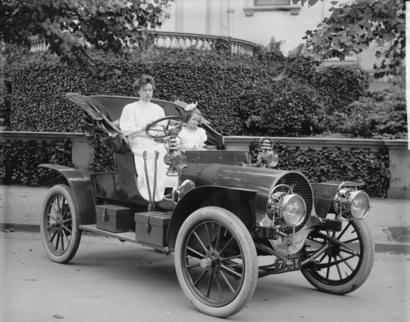
\includegraphics[width=\linewidth]{figures/sample-franklin}
	\caption{1907 Franklin Model D roadster. Photograph by Harris \&
		Ewing, Inc. [Public domain], via Wikimedia
		Commons.}
\end{figure}

Your figures should contain a caption which describes the figure to the reader.

Figure captions are placed {\itshape below} the figure.

Every figure should also have a figure description unless it is purely decorative. These descriptions convey what’s in the image to someone who cannot see it. They are also used by search engine crawlers for indexing images, and when images cannot be loaded.

\subsection{Citations and Bibliographies}

The use of BibTeX for the preparation and formatting of one's references is strongly recommended. Authors' names should be complete --- use full first names (``Donald E. Knuth'') not initials (``D. E. Knuth'') --- and the salient identifying features of a reference should be included: title, year, volume, number, pages, article DOI, etc.

The bibliography is included in your source document with these two commands, placed just before the \verb|\end{document}| command:
\begin{verbatim}
\bibliographystyle{unsrtnat}
\bibliography{bibfile}
\end{verbatim}
where ``\verb|bibfile|'' is the name, without the ``\verb|.bib|'' suffix, of the BibTeX file.

Some examples.  A paginated journal article \cite{Abril07}, an enumerated journal article \cite{Cohen07}, a reference to an entire issue \cite{JCohen96}, a monograph (whole book) \cite{Kosiur01}, a monograph/whole book in a series (see 2a in spec. document) \cite{Harel79}, a divisible-book such as an anthology or compilation \cite{Editor00} followed by the same example, however we only output the series if the volume number is given \cite{Editor00a} (so Editor00a's series should NOT be present since it has no vol. no.), a chapter in a divisible book \cite{Spector90}, a chapter in a divisible book in a series \cite{Douglass98}, a multi-volume work as book \cite{Knuth97}, a couple of articles in a proceedings (of a conference, symposium, workshop for example) (paginated proceedings article) \cite{Andler79, Hagerup1993}, a proceedings article with all possible elements \cite{Smith10}, an example of an enumerated proceedings article \cite{VanGundy07}, an informally published work \cite{Harel78}, a couple of preprints \cite{Bornmann2019, AnzarootPBM14}, a doctoral dissertation \cite{Clarkson85}, a master's thesis: \cite{anisi03}, an online document / world wide web resource \cite{Thornburg01, Ablamowicz07, Poker06}, a video game (Case 1) \cite{Obama08} and (Case 2) \cite{Novak03} and \cite{Lee05} and (Case 3) a patent \cite{JoeScientist001}, work accepted for publication \cite{rous08}, 'YYYYb'-test for prolific author \cite{SaeediMEJ10} and \cite{SaeediJETC10}. Other cites might contain 'duplicate' DOI and URLs (some SIAM articles) \cite{Kirschmer:2010:AEI:1958016.1958018}. Boris / Barbara Beeton: multi-volume works as books \cite{MR781536} and \cite{MR781537}. A couple of citations with DOIs: \cite{2004:ITE:1009386.1010128,Kirschmer:2010:AEI:1958016.1958018}. Online citations: \cite{TUGInstmem, Thornburg01, CTANacmart}. Artifacts: \cite{R} and \cite{UMassCitations}.

The bibliography is managed by the package \textbf{natbib}\footnote{\url{https://www.overleaf.com/learn/latex/Bibliography_management_with_natbib}}.


\end{document}
